
\documentclass[12pt, a4paper]{article}

\usepackage[utf8]{inputenc}
\usepackage[T1]{fontenc}
\usepackage[russian]{babel}
\usepackage[oglav,spisok,boldsect,eqwhole,figwhole,hyperref,hyperprint]{./style/fn2kursstyle}

\graphicspath{{./style/}{./figures/}}

% Параметры титульного листа
\title{Исследование устойчивости\\ некоторых течений вязкой жидкости}
\author{Ю.\,А.~Измайлова}
\supervisor{И.\,К.~Марчевский}
\group{ФН2-41Б}
\date{2020}

% Переопределение команды \vec, чтобы векторы печатались полужирным курсивом
\renewcommand{\vec}[1]{\bi{#1}}


\begin{document}

\maketitle

\tableofcontents

\newpage

\section-{Введение}

Найти, аналитически решение системы дифференциальных уравнений, описывающей течение вязкой жидкости~\cite{Loyts}, в общем случае невозможно. Только в некоторых простейших частных случаях, соответствующих довольно простым течениям, эти уравнения допускают аналитические решения. Задачи, имеющие практическое значение, решаются в основном с помощью приближенных численных методов на ЭВМ.

Основная трудность аналитического решения этих уравнений обусловлена наличием нелинейного члена, который имеет вид $ (\vec V\cdot\nabla)\vec V$, где $\vec V$ --- векторное поле скоростей жидкости. В данной работе будут рассмотрены простейшие стационарные течения, \looser{-0.02}{для которых нелинейный член тождественно равен нулю}: \emph{течения Пуазейля\footnote{Жан Луи Мари Пуазейль (\textit{фр.} Jean L\'eonard Marie Poiseuille, 1797--1869) --- французский врач и физик.}} и \emph{течения Куэтта\footnote{Морис Мари Альфред Куэтт (\textit{фр.} Maurice Marie Alfred Couette, 1858--1943) --- французский механик.}}.

Традиционно к \emph{течениям Пуазейля} относят такие стационарные течения вязкой жидкости, которые возникают в результате действия внешних сил (объемных сил или сил давления), например, при создании разности давления на концах горизонтальной трубки.
Стационарные течения, вызванные перемещением стенок, ограничивающих жидкость, называют \emph{течениями Куэтта}.

\section{Постановка задачи}

Течение вязкой несжимаемой жидкости описывается системой дифференциальных уравнений в частных производных. Уравнения движения представляют собой \emph{закон сохранения массы}, который для несжимаемой среды принимает вид
\begin{equation}
 \label{cont}
 \nabla\cdot\vec V = 0,
\end{equation}
где $\vec V = \vec V(\vec r,\, t)$ --- поле скоростей, и \emph{закон сохранения импульса}, выражение для которого называют \emph{уравнениями Навье\footnote{Клод Луи Мари Анри Навье (\textit{фр.} Claude Louis Marie Henri Navier, 1785--1836) --- французский механик и инженер.} "--- Стокса\footnote{Джордж Габриель Стокс (\textit{англ.} George Gabriel Stokes, 1819--1903) --- английский математик, механик и физик-теоретик ирландского происхождения.}}~\cite{Loyts}:
\begin{equation}
 \label{ns}
 \frac {\partial \vec V}{\partial t} + (\vec V\cdot\nabla)\vec V = -\frac{\nabla p}{\rho}+\nu\Delta\vec V.
\end{equation}
Здесь $p = (\vec r,\, t) $ --- поле давления; $\rho$ --- плотность среды, которую будем считать постоянной; $\nu$ --- постоянный коэффициент кинематической вязкости.

\looser{-0.02}{В данной работе будем рассматривать только} \emph{установившиеся}, или \emph{стационарные} течения, т.\,е.\ такие, у которых параметры остаются неизменными во времени, поэтому в уравнениях~\eqref{ns} будут присутствовать только производные по пространственным координатам, входящие в дифференциальные операторы, а зависимость всех величин от времени в дальнейшем упоминать не будем.

Поэтому для корректной постановки задачи систему уравнений~\eqref{cont}--\eqref{ns} следует дополнить граничными условиями, которыми являются \emph{условия прилипания} жидкости к твердой стенке (границе области течения):
\begin{equation}
 \vec V (\vec r)= \vec{V_\mi{K}}(\vec r), \quad \vec r \in K,
\end{equation}
где $\vec{V_\mi{K}}(\vec r)$ --- скорость движения точки с радиус-вектором $\vec r$ на границе области течения $K$.

В поставленной задаче давление в уравнении~\eqref{ns} входит только под знаком градиента, что означает невозможность его определения с точностью до константы. Поэтому задачу можно рассматривать двояко:
\begin{itemize}
\item \looser{-0.02}{задать произвольное значение давления в любой (одной) точке области течения};
\item полагать, что неизвестной величиной является не само давление, а компоненты его градиента.
\end{itemize}

\medskip

\underline{Целью} настоящей работы является получение точных решений уравнений движения вязкой несжимаемой жидкости в тех случаях, когда течение оказывается одномерным, т.\,е.\ его характеристики зависят от одной пространственной переменной. К таковым относятся так называемые течения Пуазейля и Куэтта. Также требуется рассмотреть задачу об исследовании устойчивости течения Куэтта в упрощенном безынерционном приближении.


\section{Стационарные одномерные задачи для уравнения Навье --- Стокса}

Под одномерными задачами далее будем понимать такие, в которых искомая величина зависит только от одной пространственной переменной. При этом с <<геометрической>> точки зрения такие задачи могут быть также и двумерными, и трехмерными. Далее рассмотрим четыре таких задачи: течение в плоском слое, течение в~трубе, течение в полой трубе, течение между соосными вращающимися цилиндрами.
Для каждого из рассматриваемых случаев требуется найти решение для поля скоростей и распределение давления в области течения, а также вычислить необходимые характеристики течения: расход среды, суммарную силу трения о стенки.

\subsection{Течение Пуазейля в плоском слое}
Рассмотрим стационарное течение несжимаемой жидкости, описываемое уравнениями~\eqref{cont}--\eqref{ns}, в плоском слое, как указано на рис.~\ref{planeflow1}, т.\,е.\ в зазоре между двумя неподвижными плоскостями.

\begin{figure}[!h]
\centering
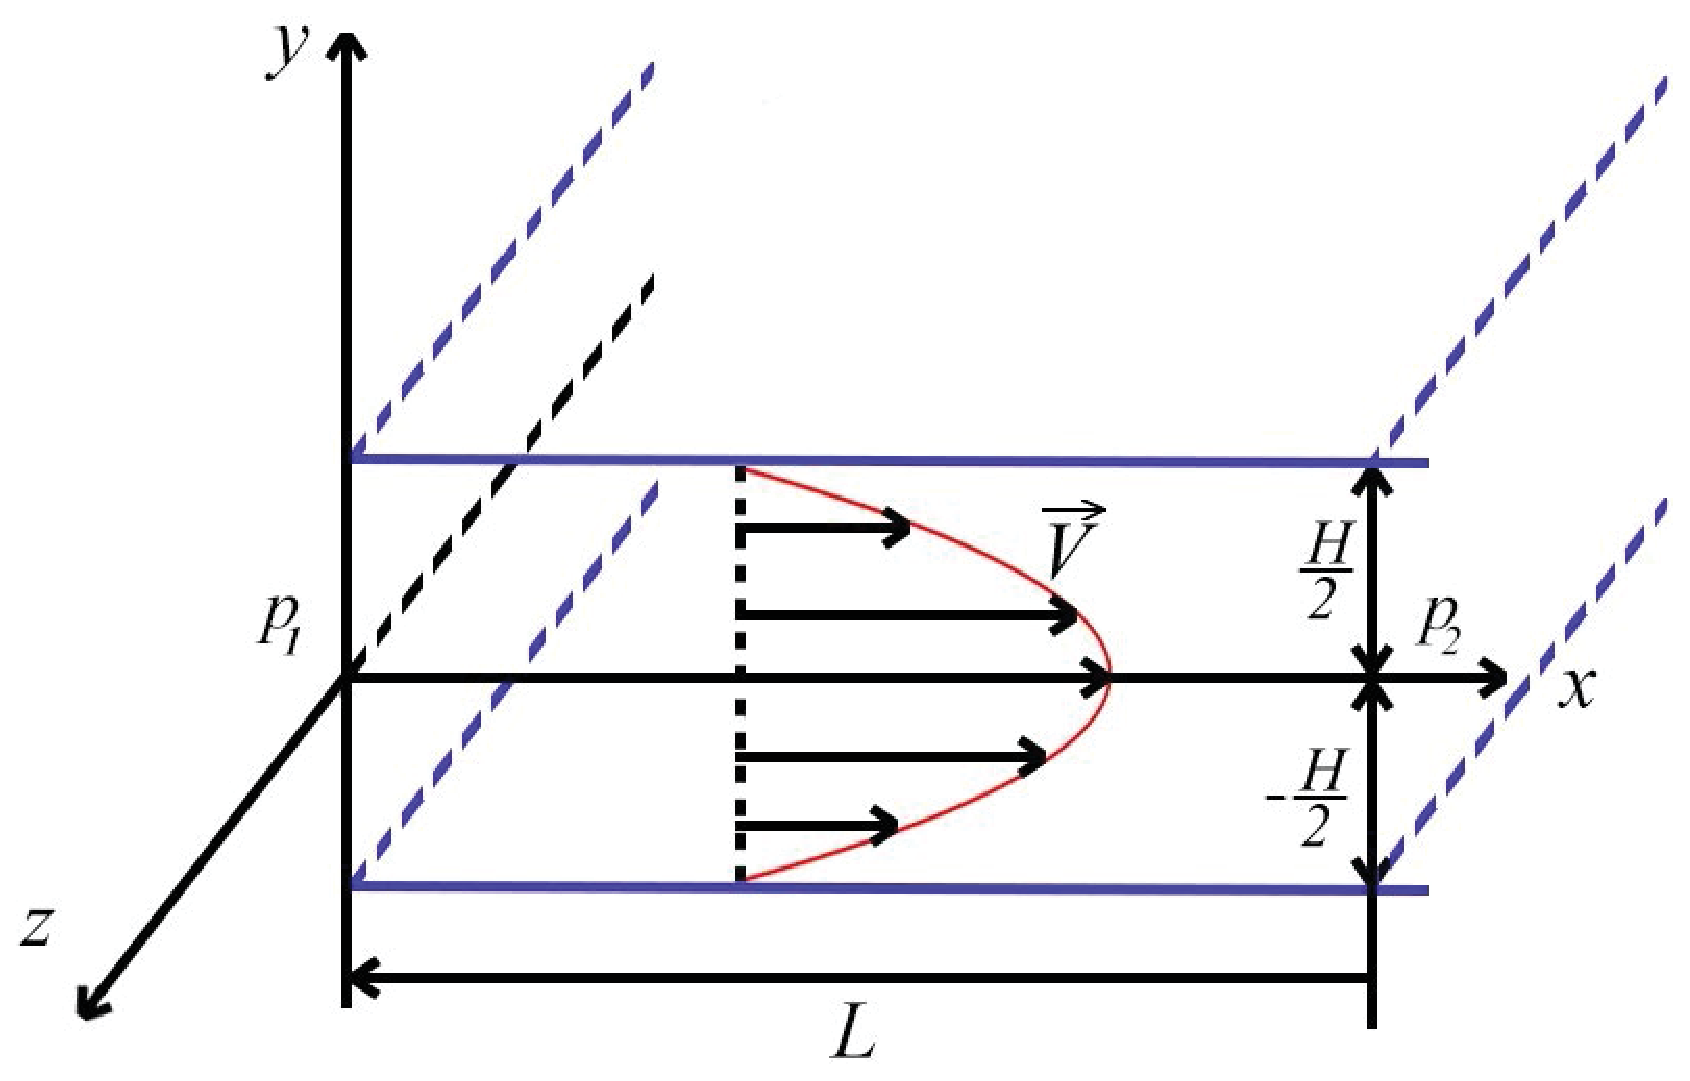
\includegraphics[width=0.45\linewidth]{planeflow1}
\caption{Течение Пуазейля в плоском слое}\label{planeflow1}
\end{figure}

Направления осей координат показаны на рис.~\ref{planeflow1}; течение предполагается плоскопараллельным, т.\,е.\ компонента скорости $V_z$ равна нулю и все характеристики течения не зависят от координаты $z$.

Предположим, что на левой и правой границах области течения задано постоянное давление, и будем дополнительно считать, что давление зависит лишь от координаты $x$, т.\,е.\ остается постоянным в любом поперечном сечении канала, $p=p(x)$. Вместе с этим, считаем, что поле скоростей во всех сечениях одинаково, значит,
\[
\frac{\partial V_x}{\partial x}=\frac{\partial V_y}{\partial x}=0.
\]
Последнее означает, что $V_x$ и $V_y$ если зависят, то только от одной переменной $y$.


Таким образом, можно записать граничные условия для данной задачи:
\[
p|_{x=0} = p_1, \quad p|_{x=L} = p_2, \quad V_x|_{y=-H/2}=V_x|_{y=H/2}=0, \quad  V_y|_{y=-H/2}=V_y|_{y=H/2}=0.
\]

С учетом сделанных предположений уравнения~\eqref{cont}--\eqref{ns} принимают вид
\begin{equation}
\label{system}
\begin{cases}
\dfrac{1}{\rho}\dfrac{dp}{dx}=\nu \dfrac{d^2V_x}{dy^2},\\
0=\nu \dfrac{d^2 V_y}{dy^2},\\
\dfrac{dV_y}{dy}=0.
\end{cases}
\end{equation}
Поскольку $\sfrac{dV_y}{dy}=0$, то $V_y=\mathrm{const}$. Принимая во внимание граничные условия
\[
V_y|_{y=-H/2}=V_y|_{y=H/2}=0,
\]
получаем, что  $V_y \equiv 0$.

\pagebreak

Отличная от нуля компонента скорости направлена вдоль оси $Ox$, так же направлен и градиент давления. Соответственно, получим следующие зависимости:
\[
	V_x=V_x(y);\quad	V_y=V_z\equiv 0; \quad 	p=p(x).
\]


Продифференцируем первое из системы уравнений~\eqref{system} по $x$:
\[
	\frac{d^2p}{dx^2}=0.
\]
\looser{-0.03}{Решая его, получаем} $p=C_1x+C_2$; \looser{-0.03}{а с учетом граничных условий для давления находим}
\begin{equation}
\label{solp}
	p(x) = p_1 + \frac{p_2-p_1}{L}x, \qquad \frac{dp}{dx}=\frac{p_2-p_1}{L} = \mathrm{const}.
\end{equation}
\looser{-0.02}{Решая теперь первое из уравнений}~\eqref{system} относительно $V_x=V_x(y)$ с учётом~\eqref{solp}, получаем:
\[
	V_x(y)=\frac{1}{\rho\nu}\frac{p_2-p_1}{L}\frac{y^2}{2}+C_3y+C_4.
\]
Значения констант $C_3$ и $C_4$ находим из граничных условий $V_x|_{-H/2} = V_x|_{-H/2} = 0$:
\[
	\begin{cases}
			0=\dfrac{1}{\rho\nu}\dfrac{p_2-p_1}{L}\dfrac{H^2}{8}+C_3\dfrac{H}{2}+C_4,\\[3mm]
			0=\dfrac{1}{\rho\nu}\dfrac{p_2-p_1}{L}\dfrac{(-H)^2}{8}-C_3\dfrac{H}{2}+C_4,
   \end{cases}\\
\]
откуда находим
\[
 C_3 = 0, \qquad C_4 =-\frac{1}{\rho\nu}\frac{p_2-p_1}{L}\frac{H^2}{8}
\]

Окончательно решение исходной системы~\eqref{cont}--\eqref{ns} с учетом граничных условий и~принятого обозначения $\mu = \rho \nu$ для динамической вязкости имеет вид
\begin{gather}\label{eq3}
V_x(y)=\frac{1}{2\mu}\frac{p_1-p_2}{L}\left(\frac{H^2}{4}-y^2\right),\\
p(x)=p_1 + \frac{p_2-p_1}{L}x.
\end{gather}

Такое поле скоростей называется плоским течением Пуазейля и применяется для описания ламинарного течения в плоских прямоугольных каналах, в которых один поперечный размер много больше другого.

Теперь найдем объемный расход жидкости, т.\,е.\ объем среды, протекающий через поперечное сечение канала между пластинами в единицу времени (в расчете на единицу длины вдоль направления $Oz$), по формуле
\begin{multline*}
 Q=\int\limits_{-H/2}^{H/2} V_x(y)\, dy = \int\limits_{-{H/2}}^{H/2}\frac{1}{2\mu}\frac{p_1-p_2}{L}\left(\frac{H^2}{4}-y^2\right) dy={}\\
 {}=\frac{p_1-p_2}{2\mu L}\left.\left(\frac{H^2y}{4}-\frac{y^3}{3}\right)\right|_{-H/2}^{H/2}=\frac{p_1-p_2}{\mu L}\frac{H^3}{12}.
\end{multline*}

Напряжение трения (т.\,е.\ сила трения протекающей жидкости о стенку в расчете на единицу площади стенки) вычисляется по формуле
\[
		\tau = \left.\mu\frac{\partial V_x}{\partial \vec n}\right|_w,
\]
где $\vec n$ --- орт нормали, направленный от стенки в сторону жидкости; нижний индекс~$w$ означает, что производная вычисляется на стенке.
Тогда на нижней стенке
\[
\tau|_{y=-H/2} = \left.\mu\frac{\partial V_x}{\partial y}\right|_{y=-H/2} = \frac{p_1-p_2}{2L}H,
\]
и на верхней стенке		
\[
 \tau|_{y= H/2} = \left.-\mu\frac{\partial V_x}{\partial y}\right|_{y=H/2} = \frac{p_1-p_2}{2L}H.
\]

Суммарная сила трения:
\[
F_{vis} = \bigl(\tau|_{y= H/2}+\tau|_{y=-H/2}\bigr)L=(p_1-p_2)H.
\]
Видно, что сила трения в данной задаче представляет разность силы давления, которое оказывается на жидкость на входе в канал слева, и силы давления, которое оказывает жидкость при выходе из канала справа.


\subsection{Течение Пуазейля в круглой цилиндрической трубе}

В данном разделе рассматривается стационарное течение несжимаемой жидкости, описываемое уравнениями~\eqref{cont}--\eqref{ns}, в сечении круглой цилиндрической трубы длиной~$L$, во много раз превышающей ее радиус $R$, т.\,е.\ $L\gg R$ (рис.~\ref{planeflow2}).

\begin{figure}[!h]
\centering
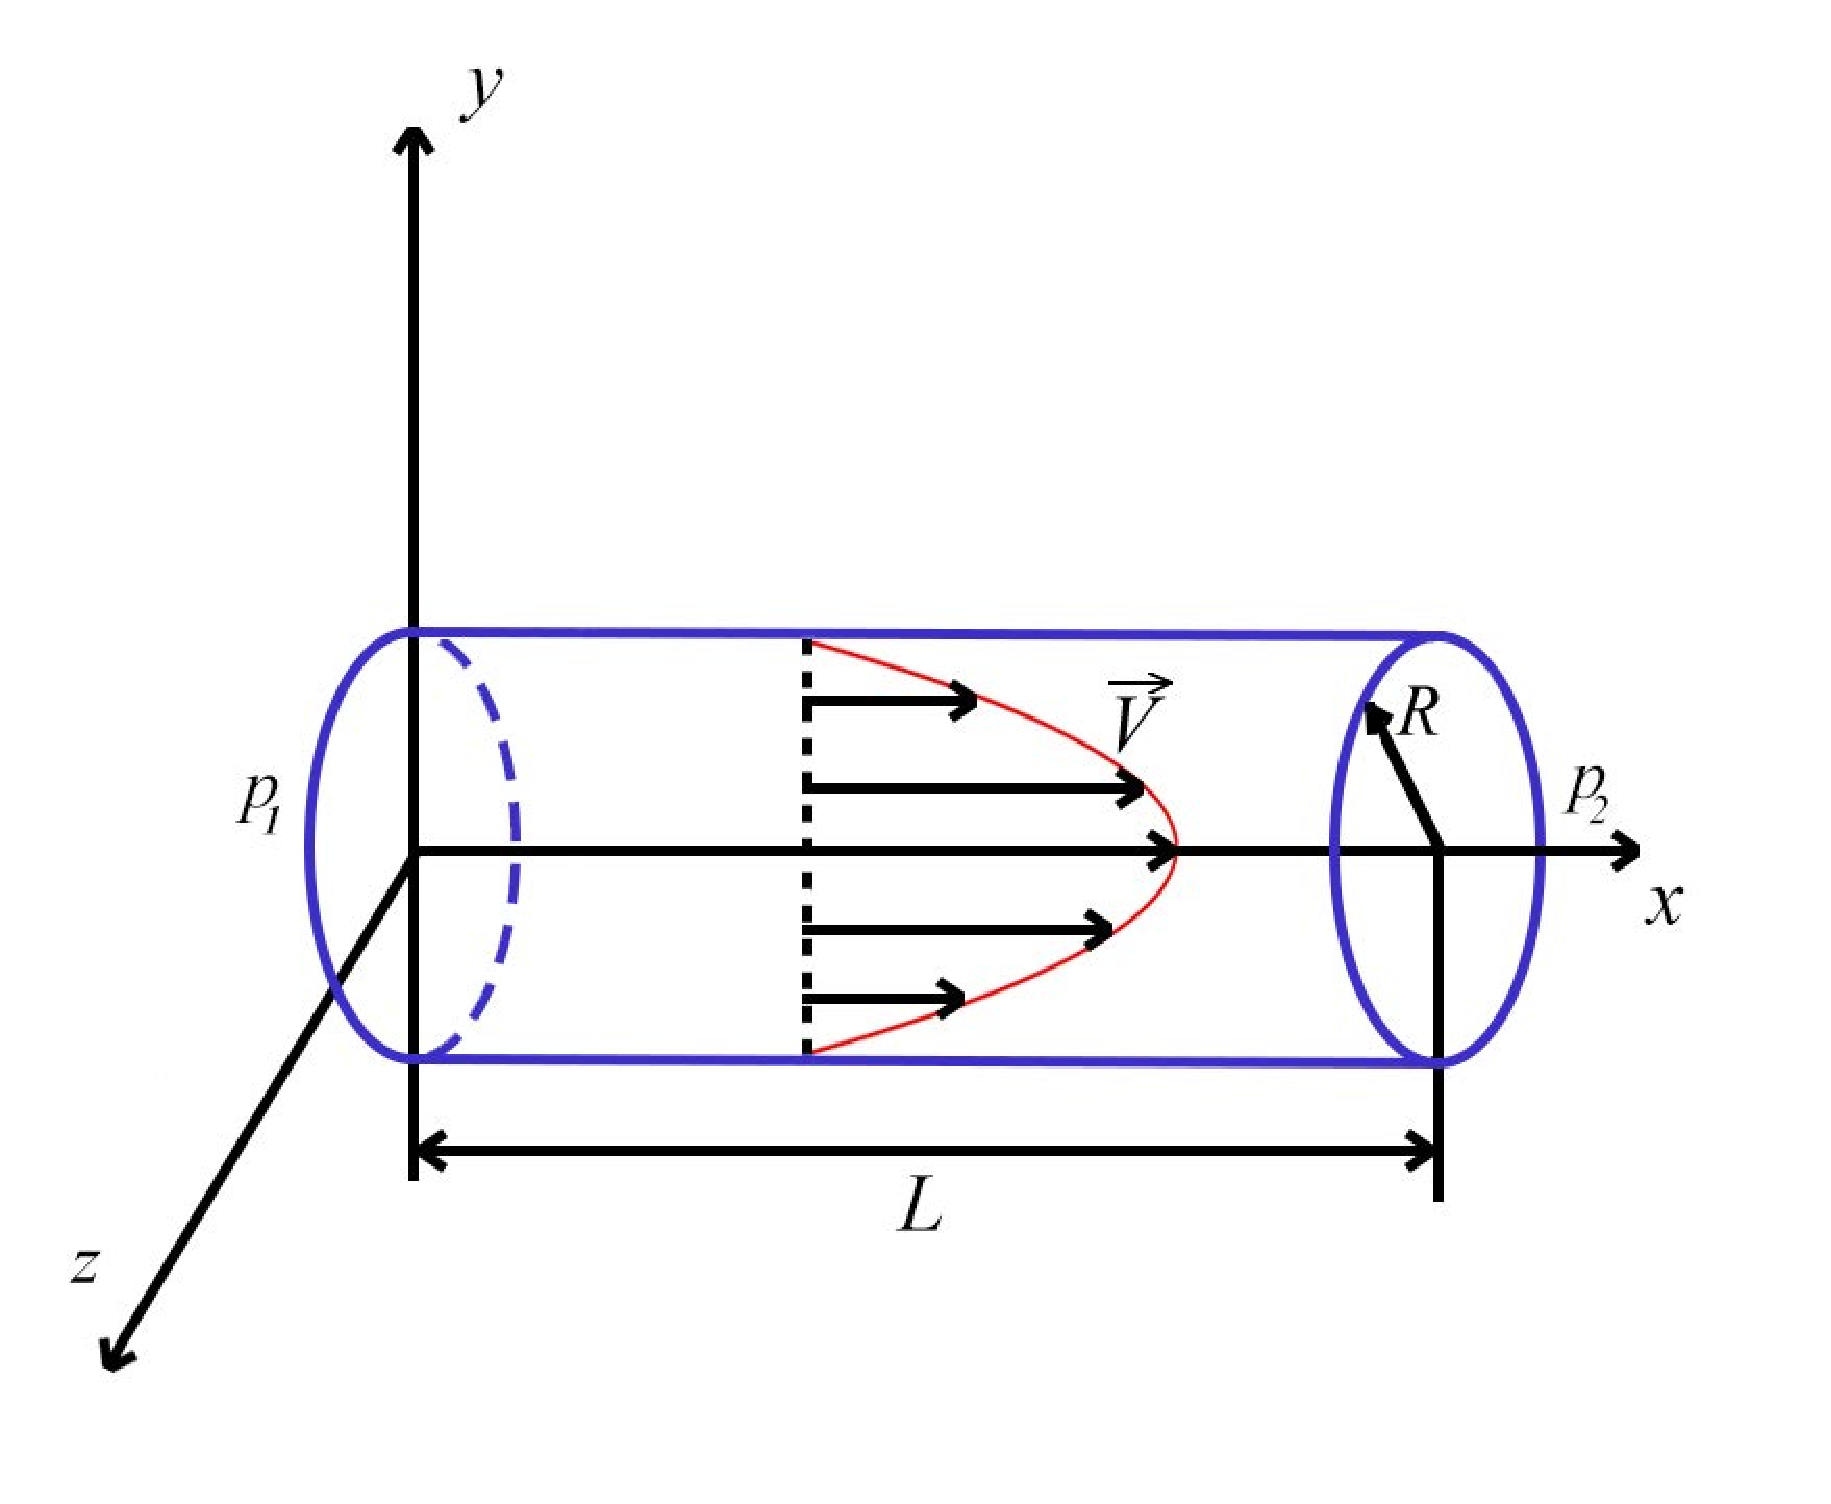
\includegraphics[width=0.55\linewidth]{planeflow2}
\caption{Течение Пуазейля в круглой трубе}\label{planeflow2}
\end{figure}

Поскольку течение в круглой трубе симметрично относительно оси цилиндра, то удобно перейти в цилиндрическую систему координат с осью $Ox$, направленной вдоль оси цилиндра. Из соображений симметрии следует, что все параметры течения не зависят от полярного угла $\phi$, и кроме того условимся рассматривать т.\,н.~\emph{незакрученные} течения, в которых $V_{\phi}\equiv0$.


В связи с тем, что $L\gg R$, трубу можно считать бесконечно длинной. Тогда течение во всех поперечных сечениях будет одинаковым и компоненты скорости не будут зависеть от пространственной координаты $x$, а производные по $x$ от этих компонент обращаются в ноль.

Труба представляет собой круговой цилиндр, поэтому рационально предположить, что радиальная компонента скорости $V_r$ равна нулю, $V_r\equiv0$. Тогда для скорости $V$ справедлива следующая зависимость:
\[
	V_x=V_x(r), \quad V_{\phi}=V_r\equiv0.
\]

Из-за осевой симметрии течения давление $p$ тоже не будет зависеть от угловой компоненты $\phi$. Дополнительно считаем, что давление остается постоянным в любом поперечном сечении канала и меняется только по его длине: $p=p(x)$.

Запишем граничные условия для данной задачи с учетом того, что течение создается и поддерживается постоянной разностью давлений:
\[
 p|_{x=0} = p_1, \quad p|_{x=L} = p_2, \quad	V_x(R)=0.
\]

В уравнении~\eqref{ns} нелинейное слагаемое $(\vec V\cdot\nabla)\vec V=0$, потому что данное выражение имеет смысл производной векторного поля $\vec V$ в направлении этого же вектора $\vec V$, умноженной на норму~$\|\vec V\|$; выше было отмечено, что $\vec V$ имеет только продольную компоненту, которая при этом не зависит от продольной координаты.
Тогда система уравнений~\eqref{cont}--\eqref{ns} примет вид:
\begin{equation}
\label{syscyl}
\begin{cases}
	\nabla\cdot\vec V=0,\\
	\dfrac{\nabla p}{\rho}=\nu\Delta\vec V.
	\end{cases}
\end{equation}
Воспользуемся формулами, через которые выражаются дифференциальные операторы $\nabla$ и $\Delta$ в цилиндрической системе координат.
\begin{itemize}
\item Оператор градиента:
\begin{equation}
\label{nabla}
\nabla\Phi =\frac{\partial\Phi}{\partial r}\,\vec e_r +\frac{1}{r}\frac{\partial\Phi}{\partial\phi}\,\vec e_{\phi}+\frac{\partial\Phi}{\partial x}\,\vec e_x.
\end{equation}
\item Лапласиан скалярной функции:
\begin{equation}
\label{Lscalar}
\Delta\Phi  = \frac{1}{r}\frac{\partial}{\partial r}\left( r\frac{\partial\Phi}{\partial r} \right) + \frac{1}{r^2}\frac{\partial^2\Phi}{\partial\phi^2}+\frac{\partial^2\Phi}{\partial x^2}.
\end{equation}
\item Лапласиан векторной функции:
\begin{equation}
\label{Lvec}
\Delta \vec F =\left(\Delta F_r-\frac{F_r}{r^2}-\frac{2}{r^2}\frac{\partial F_{\phi}}{\partial\phi}\right)\vec e_r + \left(\Delta F_{\phi}-\frac{F_{\phi}}{r^2}+\frac{2}{r^2}\frac{\partial F_r}{\partial\phi}\right)\vec e_{\phi}+(\Delta F_x)\,\vec e_x.
\end{equation}
\end{itemize}
Здесь $\vec e_r$, $\vec e_\phi$ и $\vec e_x$ --- базисные векторы в цилиндрической системе координат в соответствующей точке.


Рассмотрим $\nabla p$ с учётом~\eqref{nabla} и $p=p(x)$:\rem{Проверить Лапласиан!}
\begin{equation}
\label{gradp}
	\nabla p=\underbrace{\frac{\partial p}{\partial r}}_0\vec e_r+\frac{1}{r}\underbrace{\frac{\partial p}{\partial \phi}}_0\vec e_{\phi} + \frac{\partial p}{\partial x}\,\vec e_x=\frac{\partial p}{\partial x}\,\vec e_x.
\end{equation}
Рассмотрим $\Delta\vec V$ с учётом~\eqref{Lscalar}--\eqref{Lvec}, а также   $V_x=V_x(r)$, $V_r=V_{\phi}\equiv 0$:
\begin{equation}
\label{laplv}
	\Delta\vec V= (\Delta V_x)\vec {e_x}=
\left(\frac{1}{r}\frac{\partial}{\partial r}\left(r\frac{\partial V_x}{\partial r}\right)+\frac{1}{r^2}\underbrace{\frac{\partial^2 V_x}{\partial {\phi^2}}}_0+\underbrace{\frac{\partial^2 V_x}{\partial {x^2}}}_0\right)\!\vec e_x=\frac{1}{r}\frac{\partial}{\partial r}\left(r\frac{\partial V_x}{\partial r}\right) \vec e_x.
\end{equation}
Тогда второе из системы уравнений~\eqref{syscyl}, исходя из~\eqref{gradp} и~\eqref{laplv}, будет иметь вид (далее производные обозначаем полными, т.\,к.\ соответствующие величины зависят только от одной переменной)
\begin{equation}\label{eq5}
	\frac{1}{\rho}\frac{dp}{dx}=\nu\frac{1}{r}\frac{d}{dr}\left(r\frac{dV_x}{dr}\right).
\end{equation}
Поскольку давление остается постоянным в любом поперечном сечении канала, а~скорость жидкости не зависит от координаты $x$, значит, аналогично предыдущей задаче, можно установить, что
\begin{equation}
\label{solp1}
p(x) = p_1 + \frac{p_2-p_1}{L}x, \qquad \frac{dp}{dx}=\frac{p_2-p_1}{L} = \mathrm{const}.
\end{equation}
Таким образом, задача свелась к решению обыкновенного дифференциального уравнения.
Решая~\eqref{eq5} относительно $V_x=V_x(r)$ с учетом~\eqref{solp1}, получаем:\rem{Не бывает логарифмов размерных величин, необходимо переформулировать!}
\begin{equation*}
V_x(r)=\frac{p_2-p_1}{4\mu L}r^2+C_3\ln{r}+C_4.
\end{equation*}

Постоянную $C_3$ следует положить равной нулю, т.\,к.\ иначе будет нарушаться понятное из физического смысла задачи условие конечности скорости жидкости $V_x(0)<\infty$.\\

Постоянную $C_4$ находим из условия $V_x(R)=0$:
\begin{equation*}
0=\frac{p_2-p_1}{4\mu L}R^2+C_4,\qquad\mbox{откуда}\qquad C_4=\frac{p_1-p_2}{4\mu L}R^2.
\end{equation*}
Окончательно получаем решение уравнения~\eqref{eq5}:
\begin{gather}
V_x(r)=\frac{p_1-p_2}{4\mu L}(R^2-r^2),\\
p(x) = p_1 + \frac{p_2-p_1}{L}x.
\end{gather}
Аналогично предыдущей задаче найдем основные характеристики течения.

Объемный расход жидкости:
\begin{equation}
\label{Q1}
	Q=\int\limits_{0}^{R} V_x(r)\cdot 2\pi r dr=\frac{\pi(p_1-p_2)}{2\mu L}\left(\frac{R^4}{2}-\frac{R^4}{4}\right)=\frac{\pi(p_1-p_2)}{8\mu L}R^4.
\end{equation}
Из формулы видно, что расход жидкости прямо пропорционален перепаду давления, радиусу трубы в 4-ю степень, и обратно пропорционален коэффициенту динамической вязкости $\mu$. Формулу~\eqref{Q1} используют для экспериментального определения коэффициента $\mu$.

Напряжение трения на стенке трубы:\rem{Кажется, что должно быть $\frac{\partial V_x}{\partial \vec n}$}
\[
	\tau=-\rho\nu\left.\frac{d V_x}{d r}\right|_R=\frac{(p_1-p_2)}{2L}R.
\]

Сила вязкого трения на стенке трубы:
\[
	F=\tau\cdot 2\pi RL=\frac{(p_1-p_2)}{2L}R\cdot 2\pi RL=(p_1-p_2)\pi R^2.
\]

Как и при рассмотрении течения в плоском канале, сила трения равна разности силы давления на входе и на выходе из трубы. Иными словами, сила, приложенная к жидкости слева, <<распределяется>> между силой давления жидкости на выходе из трубы и силой трения жидкости о стенки трубы.

\newpage

\begin{thebibliography}{9}
\bibitem{Loyts} Лойцянский Л.\,Г. Механика жидкости и газа. М.: Дрофа, 2003. 846 с.
\end{thebibliography}

\end{document}
